\documentclass{beamer}
\mode<presentation>
\usetheme{CambridgeUS}
\usepackage[russian]{babel}
\usepackage[utf8]{inputenc}
\usepackage[T2A]{fontenc}
\usepackage{sansmathaccent}

\usepackage{verbatim}
\usepackage{alltt}

\pdfmapfile{+sansmathaccent.map}
\title[Язык C]{Управление процессами, часть 6}
\author{Наумов Д.А., доц. каф. КТ}
\date[15.10.2019] {Операционные системы и системное программное обеспечение, 2019}

\begin{document}

%ТИТУЛЬНЫЙ СЛАЙД
\begin{frame}
  \titlepage
\end{frame}
  
%СОДЕРЖАНИЕ ЛЕКЦИИ
\begin{frame}
  \frametitle{Содержание лекции}
  \tableofcontents  
\end{frame}

\section{Концепция потоков в Linux}

\begin{frame}{Потоки}
\begin{block}{Потоки (threads)}
позволяют одновременно выполнять разные действия в контексте одной программы. 
\end{block}
Механизмы работы с потоками реализованы в \textit{Linux} в отдельной библиотеке \textit{Pthread}.

В рамках лекции будут рассмотрены следующие темы:
\begin{itemize}
\item Понятие потоков и их особенности.
\item Создание и завершение потока.
\item Синхронизация потоков.
\item Получение информации о потоках.
\item Обмен данными между потоками.
\end{itemize}
\end{frame}

\begin{frame}[fragile]
Когда один процесс вызывает fork(), в системе появляется другой процесс, который выполняет тот же код. Но данные, которыми манипулирует этот код, являются независимой копией данных процесса-родителя. 
\begin{alltt}
#include <stdio.h>
#include <unistd.h>
int main (void)\{
  int a = 10;
  pid\_t status = fork ();
  if (!status) \{
    a++; 
    printf ("Child's a=\%d", a);
    return 0;
  \}
  wait ();
  printf ("Parent's a=\%d", a);
  return 0;
\}
\end{alltt}
\end{frame}

\begin{frame}
\begin{block}{Процессы...}
\begin{itemize}
\item ... могут иметь общие данные, но для этого программисты обращаются к методам межпроцессного взаимодействия (interprocess communication). 
\item Межпроцессное взаимодействие подчас требует сложных манипуляций со стороны программиста.
\item В некоторых случаях плохо реализованное межпроцессное взаимодействие может стать мишенью для злоумышленников.
\end{itemize}
\end{block}
\begin{block}{Потоки}
\begin{itemize}
\item ...позволяют в рамках одной программы выполнять одновременно несколько
действий, используя при этом общие данные. 
\item ...выполняются так же, как и процессы, т. е. независимо
\end{itemize}
\end{block}
\end{frame}

\section{Создание потока}

\begin{frame}{Создание потока в Linux}
\begin{enumerate}
\item Создается функция, которая называется потоковой функцией.
\item При помощи функции pthread\_create() создается поток, в котором начинает параллельно остальной программе выполняться потоковая функция.
\item Вызывающая сторона продолжает выполнять какие-то действия, не дожидаясь завершения потоковой функции.
\end{enumerate}
Чтобы подключить библиотеку Pthread к программе, нужно передать компоновщику опцию -lpthread.
\end{frame}

\begin{frame}{Создание потока в Linux}
\begin{enumerate}
\item Создается функция, которая называется потоковой функцией.
\item При помощи функции pthread\_create() создается поток, в котором начинает параллельно остальной программе выполняться потоковая функция.
\item Вызывающая сторона продолжает выполнять какие-то действия, не дожидаясь завершения потоковой функции.
\end{enumerate}
Чтобы подключить библиотеку Pthread к программе, нужно передать компоновщику опцию -lpthread.
\begin{itemize}
\item каждый поток имеет идентификатор типа \textit{pthread\_t}
\item идентификаторы потока существуют локально в рамках текущего процесса.
\end{itemize}
\end{frame}

\begin{frame}{Создание потока в Linux}
\begin{figure}[h]
\centering
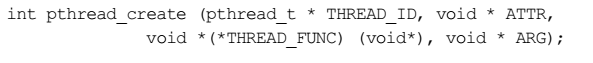
\includegraphics[scale=0.7]{images/lec08-pic01.png}
\end{figure}
Аргументы функции:
\begin{itemize}
\item THREAD\_ID - идентификатор нового потока (если таковой был создан).
\item ATTR - указание атрибутов потока. Если этот
аргумент равен NULL, то поток создается с атрибутами по умолчанию. 
\item PTHREAD\_FUNC - указатель на потоковую функцию. Это обычная функция, возвращающая бестиповый указатель (void*) и принимающая бестиповый указатель в качестве единственного аргумента.
\item ARG — указатель, содержащий аргументы потока. Если
потоковая функция не требует наличия аргументов, то в качестве ARG можно
указать NULL.
\end{itemize}
\end{frame}

\begin{frame}[fragile]{Пример nothread.c}
\begin{itemize}
\item программа при запуске создает один поток, а функция pthread\_create() позволяет создавать дополнительные потоки;
\item основную программу следует трактовать как <<родительский поток>>;
\item если один из потоков завершает программу, то все остальные потоки тут же завершаются.
\end{itemize}
\begin{alltt}
void * any_func (void * args) \{
  fprintf (stderr, "Hello World");
  sleep (5);
  return NULL;
\}
int main (void)\{
  any_func (NULL);
  fprintf (stderr, "Goodbye World");
  while (1);
  return 0;
\}
\end{alltt}
\end{frame}

\begin{frame}[fragile]{Пример thread1.c}
\begin{itemize}
\item any\_func() теперь - потоковая функция;
\item функции main() и any\_func() работают параллельно, никакой видимой задержки между выводом двух сообщений не происходит.
\end{itemize}
\begin{alltt}
void * any_func (void * args) \{...\}
int main (void)\{
  pthread_t thread;
  int result;
  result = pthread_create(&thread, NULL, &any_func, NULL);
  if (result != 0) \{
     fprintf (stderr, "Error");
     return 1;
  \}
  fprintf (stderr, "Goodbye World");
  while (1);
  return 0;
\}
\end{alltt}
\end{frame}

\begin{frame}[fragile]{Пример makefile для thread1.c}
\begin{alltt}
thread1: thread1.c
        gcc -o \$@ \$^ -lpthread
clean:
        rm -f thread1
\end{alltt}
\end{frame}

\begin{frame}[fragile]{Пример threadargs.c}
\begin{itemize}
\item Для передачи данных в поток используется четвертый аргумент функции pthread\_create();
\item Этот указатель автоматически становится аргументом потоковой функции.
\end{itemize}
\begin{alltt}
void * any_func (void * arg)
\{
    int a = *(int*) arg;
 
    fprintf (stderr, "Hello World with argument=%d", a);

    return NULL;
\}
\end{alltt}
\end{frame}

\begin{frame}[fragile]{Пример threargs.c}
\begin{alltt}
int main (int argc, char ** argv)
\{
    pthread_t thread;
    int arg, result;
    if (argc < 2) \{
        fprintf (stderr, "Too few arguments");
        return 1;
    \} 
    arg = atoi (argv[1]);
    result = pthread_create (&thread, NULL, &any_func, &arg);
    
    fprintf (stderr, "Goodbye World");
    while (1);    
    return 0;
\}
\end{alltt}
\end{frame}

\begin{frame}[fragile]{Пример threadstruct.c}
\begin{itemize}
\item Если требуется передать в поток несколько аргументов, то их можно разместить в структуре, указатель на которую также передается в потоковую функцию.
\end{itemize}
\begin{alltt}
struct thread_arg \{
    char * str;
    int num;
\};
void * any_func (void * arg)
\{
    struct thread_arg targ = (struct thread_arg *)arg;
    fprintf (stderr, "str=\%s", targ->str);
    fprintf (stderr, "num=\%d", targ->num);

    return NULL;
\}
\end{alltt}
\end{frame}

\begin{frame}[fragile]{Пример threadstruct.c}
\begin{alltt}
int main (void)\{
    pthread_t thread;
    int result;

    struct thread_arg targ;
    targ.str = "Hello World";
    targ.num = 2007;

    result = pthread_create (&thread, NULL, &any_func, &targ);

    while (1);
    return 0;
\}
\end{alltt}
\end{frame}

\section{Завершение потока}
\begin{frame}[fragile]{Пример threadexit.c}
Потоки могут завершаться: 
\begin{itemize}
\item возвратом из потоковой функции;
\item вызовом специальной функции void pthread\_exit(void * RESULT).
\end{itemize}
Если потоковая функция вызывает другие функции, то pthread\_exit() в таких случаях бывает очень полезной. 
\begin{alltt}
void print_msg (void) \{
    fprintf (stderr, "Hello World");
    pthread_exit (NULL);
\}
void * any_func (void * arg)
\{
    print_msg ();
    fprintf (stderr, "End of any_func()");
    return NULL;
\}
\end{alltt}
\end{frame}

\begin{frame}[fragile]{Пример threadexit.c}
\begin{alltt}
int main (void)
\{
    pthread_t thread;

    if (pthread_create (&thread, NULL, &any_func, NULL) != 0) 
    \{
        fprintf (stderr, "Error");
        return 1;
    \}

    while (1);
    return 0;
\}
\end{alltt}
\end{frame}

\section{Ожидание потока}
\begin{frame}[fragile]{Ожидание потока: pthread\_join()}
Функция pthread\_join() позволяет синхронизировать потоки:
\begin{alltt}
int pthread_join (pthread_t THREAD_ID, void ** DATA);
\end{alltt}
\begin{itemize}
\item функция блокирует вызывающий поток до тех пор, пока не завершится поток с идентификатором THREAD\_ID. 
\item по адресу DATA помещаются данные, возвращаемые потоком через функцию pthread\_exit() или через инструкцию return потоковой функции.
\item при удачном завершении pthread\_join() возвращает 0, любое другое значение сигнализирует об ошибке.
\end{itemize}
\end{frame}

\begin{frame}[fragile]{Пример join1.c}
\begin{alltt}
#define A_COUNT 15
#define B_COUNT 10
void * print_b (void * arg)
\{
  int i;
  for (i = 0; i < B_COUNT; i++) \{
    fprintf (stderr, "B");
    sleep (1);
  \}
  fprintf (stderr, "C");
  return NULL;
\}
\end{alltt}
\end{frame}

\begin{frame}[fragile]{Пример join1.c}
\begin{alltt}
int main (void)\{
    pthread_t thread; int i;
    if (pthread_create (&thread, NULL, &print_b, NULL) != 0) \{
      fprintf (stderr, "Error");
      return 1;
    \}
    for (i = 0; i < A_COUNT; i++) \{
      fprintf (stderr, "A");
      sleep (1);
    \}
    if (pthread_join (thread, NULL) != 0) \{
      fprintf (stderr, "Join error");
      return 1;
    \}
    fprintf (stderr, "D");
    return 0; \}
\end{alltt}
\end{frame}

\begin{frame}[fragile]{Пример join1.c}
Эта программа в течение некоторого времени выводит примерно такой "шифр":
\begin{alltt}
\$ ./join1
ABABABABABABABABABABACAAAAD
\end{alltt}
\begin{itemize}
\item Символы A печатает родительский поток. 
\item Символы B выводятся порожденным потоком. Когда этот поток завершается, выводится символ C. 
\item Когда завершается программа, печатается символ D. 
\item Кроме того, применение функции pthread\_join() наконец-то избавило нас от необходимости каждый раз запускать бесконечный цикл в конце программы.
\end{itemize}
\end{frame}

\begin{frame}[fragile]{Пример join2.c}
Пример получения данных, возвращаемых из потока.
\begin{alltt}
void * any_func (void * arg)
\{
  int a = *(int *) arg;
  a++;
  return (void *) a;
\}
\end{alltt}
\end{frame}

\begin{frame}[fragile]{Пример join2.c}
Пример получения данных, возвращаемых из потока.
\begin{alltt}
int main (void)
\{
  pthread_t thread;
  int parg = 2007, pdata;
  if (pthread_create (&thread, NULL, 
          &any_func, &parg) != 0) \{
    fprintf (stderr, "Error");
    return 1;
  \}
  pthread_join (thread, (void *) &pdata);
  printf ("%d", pdata);
  return 0;
\}
\end{alltt}
\end{frame}

\begin{frame}[fragile]{Пример join3.c}
Функцию pthread\_join() может вызывать любой поток, работающий внутри текущего процесса.
\begin{alltt}
#define A_COUNT 10
#define B_COUNT 25
#define C_COUNT 10
void * print_b (void * arg)
\{
  int i;
  for (i = 0; i < B_COUNT; i++) \{
    fprintf (stderr, "B");
    sleep (1);
  \}
  fprintf (stderr, "(end-of-B)");
  return NULL;
\}
\end{alltt}
\end{frame}

\begin{frame}[fragile]{Пример join3.c}
\begin{alltt}
void * print_c (void * arg)
\{
  pthread_t thread = * (pthread_t *) arg;
  int i;
  
  for (i = 0; i < C_COUNT; i++) \{
    fprintf (stderr, "C");
    sleep (1);
  \}
  
  fprintf (stderr, "(end-of-C)");
  pthread_join (thread, NULL);
  
  return NULL;
\}
\end{alltt}
\end{frame}

\begin{frame}[fragile]{Пример join3.c}
\begin{alltt}
int main (void)\{
  pthread_t thread1, thread2; int i;
  if (pthread_create (&thread1, NULL, &print_b, NULL) != 0) 
    return 1;
  if (pthread_create (&thread2, NULL, &print_c, &thread1) != 0) 
    return 1;
  for (i = 0; i < A_COUNT; i++) \{
    fprintf (stderr, "A");
    sleep (1);
  \}
  fprintf (stderr, "(end-of-A)");
  pthread_join (thread2, NULL);
  fprintf (stderr, "(end-of-all)");
  return 0;
\}
\end{alltt}
\end{frame}

\section{Получение информации о потоке}

\begin{frame}[fragile]{Получение информации о потоке: pthread\_self(), pthread\_equal()}
Это функция pthread\_self() возвращает идентификатор текущего потока.
\begin{alltt}
pthread_t pthread_self (void);
\end{alltt}
Тип pthread\_t является целым числом, но к идентификаторам потоков не рекомендуется применять математические операции. Для сравнения идентификаторов двух потоков служит функция pthread\_equal():
\begin{alltt}
int pthread_equal (pthread_t THREAD1, pthread_t THREAD2);
\end{alltt}
\begin{itemize}
\item Если идентификаторы относятся к одному потоку, то эта функция возвращает ненулевое значение. 
\item Если THREAD1 и THREAD2 являются идентификаторами разных потоков, то pthread\_equal() возвращает 0.
\end{itemize}
\end{frame}

\begin{frame}[fragile]{Пример join4.c}
Чаще всего значение идентификатора потока необходимо для того, чтобы уберечь поток от вызова phtread\_join() для самого себя.
\begin{alltt}
void * any_func (void * arg)
\{
  pthread_t thread = * (pthread_t *) arg;
 
  if (pthread_equal(pthread_self(), thread) != 0)
    fprintf (stderr, "1");

  return NULL;
\}
\end{alltt}
\end{frame}

\begin{frame}[fragile]{Пример join4.c}
\begin{alltt}
int main (void)
\{
  pthread_t thread;
  if (pthread_create (&thread, NULL, 
      &any_func, &thread) != 0) \{
    fprintf (stderr, "Error");
    return 1;
  \}
  if (pthread_equal (pthread_self(), thread) != 0)
    fprintf (stderr, "2");
  pthread_join (thread, NULL);
  return 0;
\}
\end{alltt}
\end{frame}

\section{Отмена потока}

\begin{frame}[fragile]{Отмена потока: pthread\_cancel()}
Любой поток может послать другому потоку запрос на завершение. 
Такой запрос называют отменой потока:
\begin{alltt}
int pthread_cancel (pthread_t THREAD_ID);
\end{alltt}
\begin{itemize}
\item Функция pthread\_cancel() возвращает 0 при удачном завершении, ненулевое значение сигнализирует об ошибке.
\item Несмотря на то, что pthread\_cancel() возвращается сразу, это вовсе не означает немедленного завершения потока.
\item В связи с этим, если для вас важно, чтобы поток был удален, нужно дождаться его завершения функцией pthread\_join().
\end{itemize}
\end{frame}

\begin{frame}[fragile]{Пример pcancel1.c}
\begin{alltt}
void * any_func (void * arg)
\{
  while (1) \{
    fprintf (stderr, ".");
    sleep (1);
  \}

  return NULL;
\}
\end{alltt}
\end{frame}

\begin{frame}[fragile]{Пример pcancel1.c}
\begin{alltt}
int main (void) \{
  pthread_t thread;
  void * result;	
  
  if (pthread_create (&thread, NULL, &any_func, NULL) != 0) 
    return 1;
    
  sleep (5);   
  pthread_cancel (thread);
  
  if (!pthread_equal (pthread_self (), thread))
    pthread_join (thread, &result);
  if (result == PTHREAD_CANCELED)
    fprintf (stderr, "Canceled");    
  return 0;
\}
\end{alltt}
\end{frame}

\section*{Дополнительная инфомация}
\begin{frame}{Дополнительная информация}
Не рассмотренные темы можно изучить на следующих страницах справочного руководства man:
\begin{itemize}
\item man pthread\_atfork;
\item man pthread\_kill;
\item man pthread\_once;
\item man pthread\_mutex\_lock; man pthread\_mutex\_unlock;
\item man pthread\_detach;
\item man pthread\_setcancelstate; man pthread\_setcanceltype; man pthread\_testcancel;
\item man pthread\_setspecific.
\end{itemize}
По приведенным далее ссылкам размещены наиболее полные руководства и источники дополнительной информации о потоках:
\begin{itemize}
\item http://yolinux.com/TUTORIALS/LinuxTutorialPosixThreads.html;
\item http://www.llnl.gov/computing/tutorials/pthreads/;
\item http://www.ibiblio.org/pub/Linux/docs/faqs/Threads-FAQ/html/;
\item http://www.humanfactor.com/pthreads/pthread-tutorials.htm
\end{itemize}
\end{frame}

\end{document}